\noindent \textred{1.}
\textbf{(4 points)} \textit{Expressivity of neural networks}. Recall that the functional form for a
single neuron is given by $y = \sigma(\langle w, x\rangle + b, 0)$, where $x$ is the input and $y$ is the output. In this exercise, assume that $x$ and $y$ are 1-dimensional (i.e., they are both just real-valued scalars) and $\sigma$ is the unit step activation. We will use multiple layers of such neurons to approximate pretty much any function $f$. There is no learning/training required for this problem; you should be able to guess/derive the weights and biases of the networks by hand.

\begin{enumerate}[a.]
    \item \label{q:1a} 
    (1pt) A \textit{box} function with height $h$ and width $\sigma$ is the function $f(x) = h$ for $0 < x < \sigma$ and 0 otherwise. Show that a simple neural network with 2 hidden neurons with step activations can realize this function. Draw this network and identify all the weights and biases. (Assume that the output neuron only sums up inputs and does not have a nonlinearity.)
    \vspace{-10pt}
    \begin{figure}[!h]
        \centering
        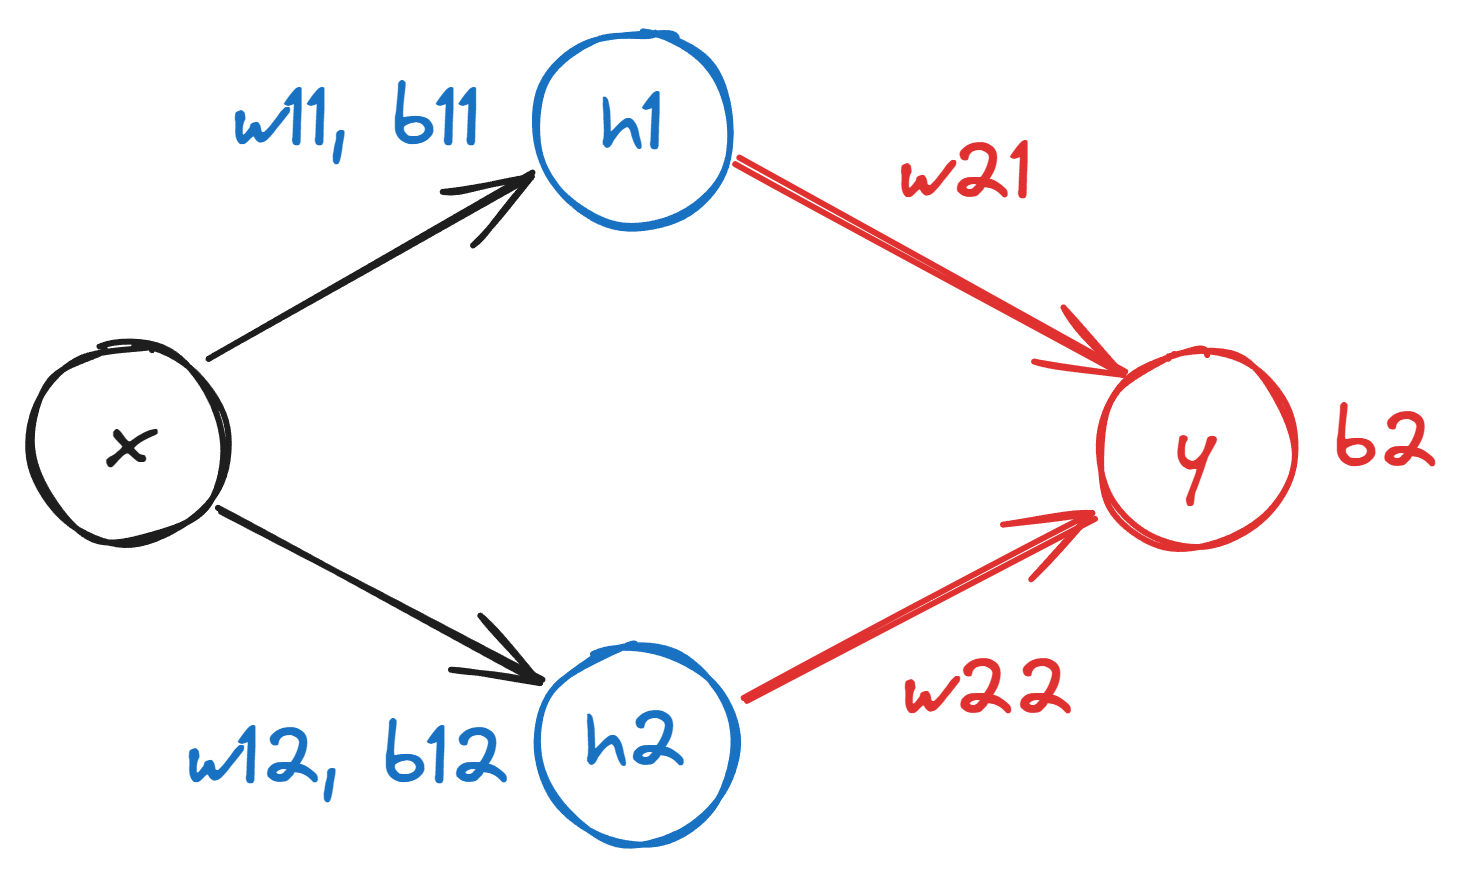
\includegraphics[width=0.4\linewidth]{HWs//HW1//figures/1.png}
    \end{figure} \\
    \myAnswer{
    There are infinite sets of weights and biases we can take to achieve the box function. \\
    For simplicity and clarity, we take \\
    $w_{11}=w_{12}=1, b_{11}=0, b_{12}=-\delta, w_{21} = -w_{22} = h, b_{2}=0$. \\
    }
    \item \label{q:1b} 
    (2pts) Now suppose that $f$ is \textit{any arbitrary, smooth, bounded} function defined over an interval $[-B, B]$. (You can ignore what happens to the function outside this interval, or just assume it is zero). Use part \ref{q:1a} to show that this function can be closely approximated by a neural network with a hidden layer of neurons. You don’t need a rigorous mathematical proof here; a handwavy argument or even a figure is okay here, as long as you convey the right intuition. \\
    \myAnswer{
    Based on the spirit of part \ref{q:1a}, we can approximate any variation of function values within any range if adjusting weights and biases very carefully. Therefore, in theory, we can divide the function within the range of $[-B, B]$ into countless small segments. For each segment, we can use a neuron (with step activation) to approximate the infinitely small variation. Combining all segments together, we obtain the whole function.
    }
    \item
    (1pt) Do you think the argument in part \ref{q:1b} can be extended to the case of $d$-dimensional inputs? (i.e., where the input $x$ is a vector – think of it as an image, or text query, etc). If yes, comment on potential practical issues involved in defining such networks. If not, explain why not. \\
    \myAnswer{
    Yes, I do. However, there could be several difficulties when defining such neural networks. 
    \begin{itemize}
        \item As input dimension increase, the high dimensional space becomes sparser than low dimensional space, which means we need to significantly increase the complexity of the neural network, \ie, the number of neurons in the hidden layer. The computational cost could be impractical.
        \item If the multi-dimensional function has strong locality, we need to carefully design the connections between inputs and hidden layer, so that different input dimensions can be disentangled. The complicated connecting situation could be impractical. \\
    \end{itemize}
    }
\end{enumerate}
